\documentclass[aspectratio=169,t]{beamer}
\usepackage[utf8]{inputenc}
\usepackage{graphicx}
\usepackage{color}
\usepackage{graphicx}
\usepackage{fancybox}
\usepackage[vlined]{algorithm2e}
\usepackage{standalone}
\usepackage{tikz}
\usetikzlibrary{shapes,arrows.meta}
%\usepackage{enumitem}

\usepackage{beamerthemesplit}
\usetheme[compress]{Heidelberg}
\definecolor{unirot}{rgb}{0.5976525,0,0}
\usecolortheme[named=unirot]{structure}

\title{GPGPU Accelerated Iterative Filtering of Scalar Fields on Discrete Manifolds}
\author{Bryan Wolfford}

\institute[Uni HD]{
	Universität Heidelberg\\
	Interdisciplinary Center for Scientific Computing\\
	Forensic Computational Geometry Laboratory\\
	\color{unirot}{wolfford@stud.uni-heidelberg.de}
}
\date{\today}

%\AtBeginSection[]{
%	\begin{frame}<beamer>
%		\frametitle{Outline}
		% show TOC and highlight current section
%		\tableofcontents[currentsection]
%	\end{frame}
%}

%\AtBeginSubsection[]{
%	\begin{frame}<beamer>
%		\frametitle{Outline}
		% show TOC and highlight current section
%		\tableofcontents[currentsection,currentsubsection]
%	\end{frame}
%}

\begin{document}
\newcommand{\fors}[1]{#1he Fast One-Ring smoothing filter}
\newcommand{\Fors}[1]{#1he Fast One-Ring smoothing filter for scalar fields on discrete manifolds}
\newcommand{\tdd}{3D-data}
\newcommand{\wmfv}[1]{weighted mean function value#1}
%
\newcommand{\bE}{\mathcal{E}}
\newcommand{\bF}{\mathcal{F}}
\newcommand{\bM}{\mathcal{M}}
\newcommand{\bN}{\mathcal{N}}
\newcommand{\bO}{\Omega}
\newcommand{\bP}{\mathcal{P}}
\newcommand{\bR}[1]{\mathbb{R}^{#1}}
\newcommand{\bT}{\mathcal{T}}
\newcommand{\bc}{\mathbf{c}}
\newcommand{\bp}{\mathbf{p}}
\newcommand{\bs}{\mathbf{s}}
\newcommand{\bt}{\mathbf{t}}
\newcommand{\bv}{\mathbf{v}}
%
\newcommand{\elm}{\ell_\text{min}}
\newcommand{\gelm}{\overline{\elm}}
\newcommand{\ellstar}{\ell_\ast}
%
\newcommand{\fM}{\mathfrak{M}}
%
\newcommand{\mbeq}{\overset{!}{=}}
%
\newcommand{\sipo}{i\kern-.7pt\scalebox{0.66}{+}\kern-1.2pt1}
\newcommand{\sipt}{i\kern-.7pt\scalebox{0.66}{+}\kern-1.2pt2}
\newcommand{\sjpo}{j\kern-.7pt\scalebox{0.66}{+}\kern-1.2pt1}
\newcommand{\sjpt}{j\kern-.7pt\scalebox{0.66}{+}\kern-1.2pt2}
\newcommand{\sps}{\kern-2pt+\kern-3pt}
\newcommand{\sxpx}[2]{#1\kern-.7pt\scalebox{0.66}{+}\kern-1.2pt#2}
\newcommand{\sv}[1]{v,\kern.75pt #1}
%
\newcommand{\todoRemove}[1]{\todo[color=red!40]{Remove: #1}}
\newcommand{\todoAsk}[1]{\todo[color=yellow!40]{Ask: #1}}
\newcommand{\todoCitation}[1]{\todo[color=teal!40]{Cite: #1}}
\newcommand{\todoReference}[1]{\todo[color=lime!40]{Ref: #1}}
\newcommand{\todoResearch}[1]{\todo[color=magenta!40]{Research: #1}}
\newcommand{\todoBackground}[1]{\todo[color=violet!40]{Bg: #1}}
\newcommand{\todoReword}[1]{\todo[color=cyan!40]{Reword: #1}}
\newcommand{\todoStyle}[1]{\todo[color=pink!40]{Style: #1}}
%xcolor base colors:
%	black
%	blue
%	brown
%%%	cyan
%%%	lime
%%%	magenta
%	olive
%	orange
%%%	pink
%	purple
%%%	red
%%%	teal
%%%	violet
%	white
%%%	yellow

\definecolor{MyTeal}{rgb}	{0, 	.5, 	.5}		%teal = 0,127,127
\definecolor{MyLtTeal}{rgb}	{.8125, .9375, 	.9375}	%lt.teal = 207,239,239
\definecolor{MySand}{rgb}	{1, 	.625, 	0}		%sand = 255,159,0
\definecolor{MyLtSand}{rgb}	{1, 	.9766, 	.875}	%lt.sand = 255,249,223
\definecolor{MyCoral}{rgb}	{1, 	.375, 	.375}	%coral = 255,96,96
\definecolor{MyLtCoral}{rgb}{1, 	.875, 	.875}	%lt.coral = 255,223,223

\setlength{\intextsep}{0pt}
\frame[plain]{\titlepage}
\frame{\frametitle{Outline}\tableofcontents}




%================================================
%================================================
\section{Motivation \& Introduction}

%------------------------------------------------
\frame{\frametitle{Motivation}
	\begin{itemize}
		\item Increasing demand for high-definition \tdd{}
		\begin{itemize}
			\item Industrial quality scanning~\cite{ILATO14}
			\item Fuzzy borders on hyroglyphs
			\item OCR
		\end{itemize}

		\item Danger to physical archives
		\begin{itemize}
			\item 2018 Brazilian museum fire destroyed 20 million artifacts~\cite{Andreoni18}
		\end{itemize}
	\end{itemize}


%\section{Motivation}
%3D-Data is important to many fields
From industrial quality scanning~\cite{ILATO14}, to computerized analysis of documents and artifacts within the Digital Humanities~\cite{Bogacz15}, the demand for high-definition \tdd{} is only increasing. And in light of recent tragedies befalling global physical archives, like the museum fire which destroyed Brazil's oldest museum and its 20 million artifacts~\cite{Andreoni18}, or the numerous war zones occupying archaeologically important sites, 3D-scanning will continue to increase in importance.

%3D-Data Noises in data, so must still process
However, raw \tdd{} is typically not suitable for analysis~\cite[p.~25-32]{Mara12}, so processing and pre-processing with a smoothing filter becomes necessary. In dense, high-resolution meshes, for example, one can see noise propagating as jagged outlines in segment boundaries of connected components when visualizing the output of filters designed for analysis, like the Multi-Scale Integral Invariants filter (MSII)~\cite[s.~3.2]{Mara17}.

%processing is difficult
One major complication slowing the development of filters for \tdd{} has been that the window size of any filter must remain static for the duration of its convolution, in order for the output response to be mapped correctly back onto the input field~\cite[p.~106-112]{Jaehne97}. While it is trivial to define a static-sized filter for convolving regular meshes like raster images, it is a complex and complicated task to create the same for convolving acquired \tdd{}, whose one-ring neighborhoods are subsets of non-planar meshes embedded in $\bR{3}$, uniformly irregular, with completely arbitrary shapes, sizes, and counts of members~\cite[p.~29]{Mara12}~\cite[s.~3.2]{Mara17}.

%3D-Data is big. serial is slow
Another problem which arises, is that with high-resolution 3D-scanning, the data output is often comprised of millions, or tens of millions, of points per scanned item and features several hundred points per mm$^2$~\cite[25,144]{Mara17}~\cite[4]{ILATO14}. At that scale, serial algorithms processing that data can no longer be included in the regular workflow of a scientist analyzing the artifacts, because each operation can easily take hours or days to complete.


%gpgpus are cheap, so do the thing
Fortunately, with the introduction of GPGPUs to the commercial market, individual research groups now have the opportunity to exploit the parallel processing power of SIMD systems, without needing access to an institutional supercomputer. Therefore, the motivation for designing a smoothing filter, which can efficiently convolve over large, irregular, acquired \tdd{} by utilizing commercially available GPGPUs, was realized. Thus came \Fors{t}, and the research presented in this thesis.
}

%------------------------------------------------
\frame{\frametitle{Introduction}

}

%------------------------------------------------
\frame{\frametitle{SIMD Architecture}
	\includegraphics[width=1.0\linewidth]{../figures/tikz/simdArchitecture.pdf}
	GPUs, Supercomputers, Computer Pools %Name examples like the cray, and pool in this building
}

%------------------------------------------------
\frame{\frametitle{CPU vs GPU Construction}
	\includegraphics[width=1.0\linewidth]{../figures/cpuvgpu.png}
}

%------------------------------------------------
\frame{\frametitle{One-Ring Neighborhoods in Regular and Irregular Meshes}
	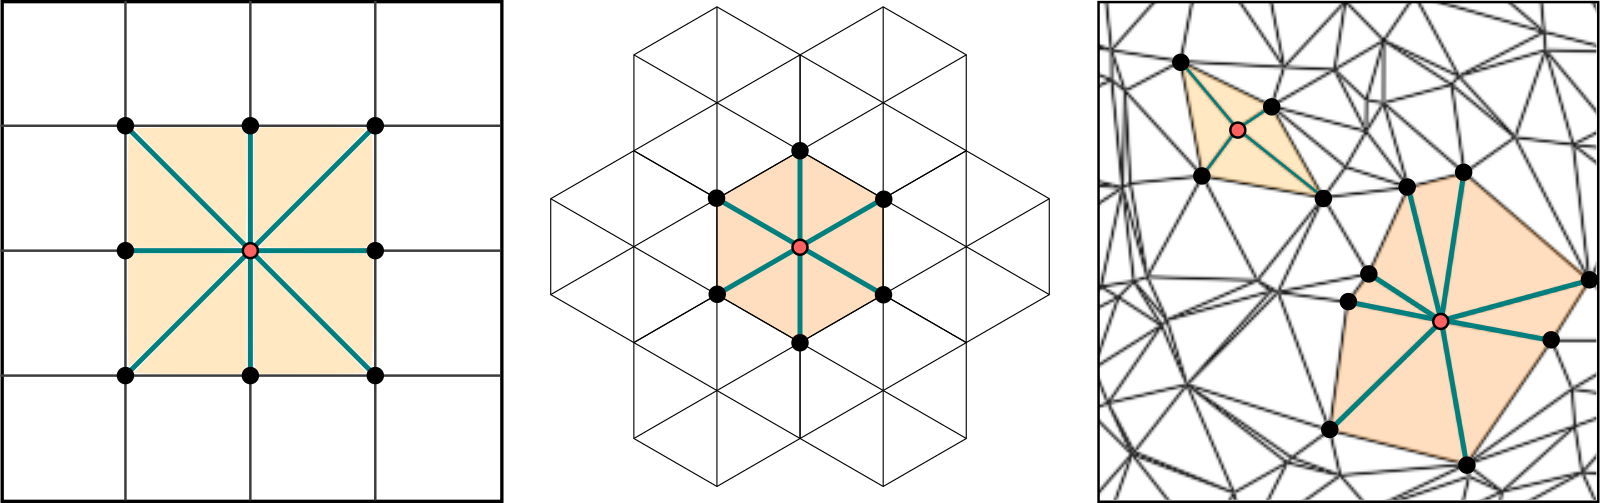
\includegraphics[width=1.0\linewidth]{../figures/neighborhoods_presentation.png}
	One-ring neighborhoods in (a) a regular square mesh, as in pixels of a digital image (b) a regular triangle mesh, as in a hexagonal tessellation (c) an irregular triangle mesh, typical of acquired \tdd{}.

}




%================================================
%================================================
\section[Fast One-Ring Smoothing]{Fast One-Ring Smoothing}


%================================================
\subsection[Foundation]{Mathematical Foundation}

%------------------------------------------------
\frame{\frametitle{A One-Ring Neighborhood and its Geodesic Disc}
	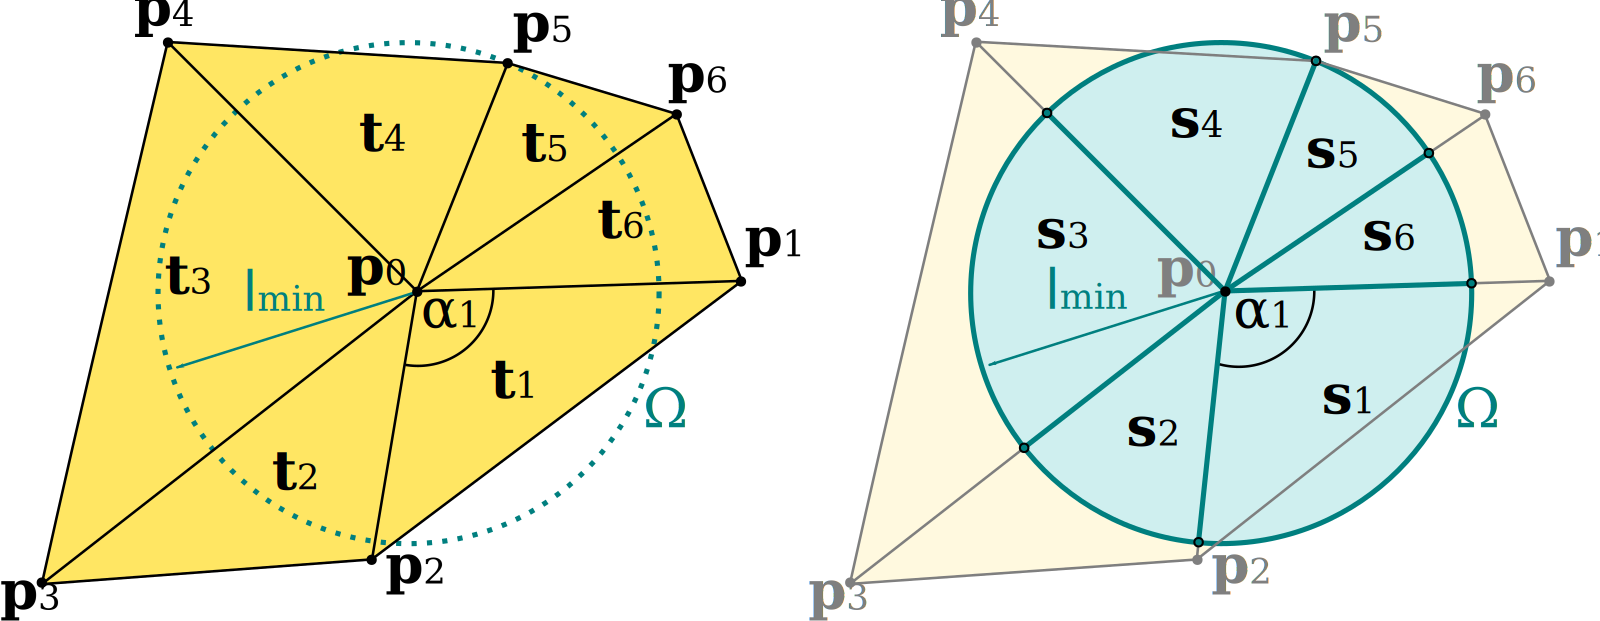
\includegraphics[width=1.0\linewidth]{../figures/geodesicDisc_presentation.png}
}

%------------------------------------------------
\frame{\frametitle{An Enhanced View of a Circle Sector}
	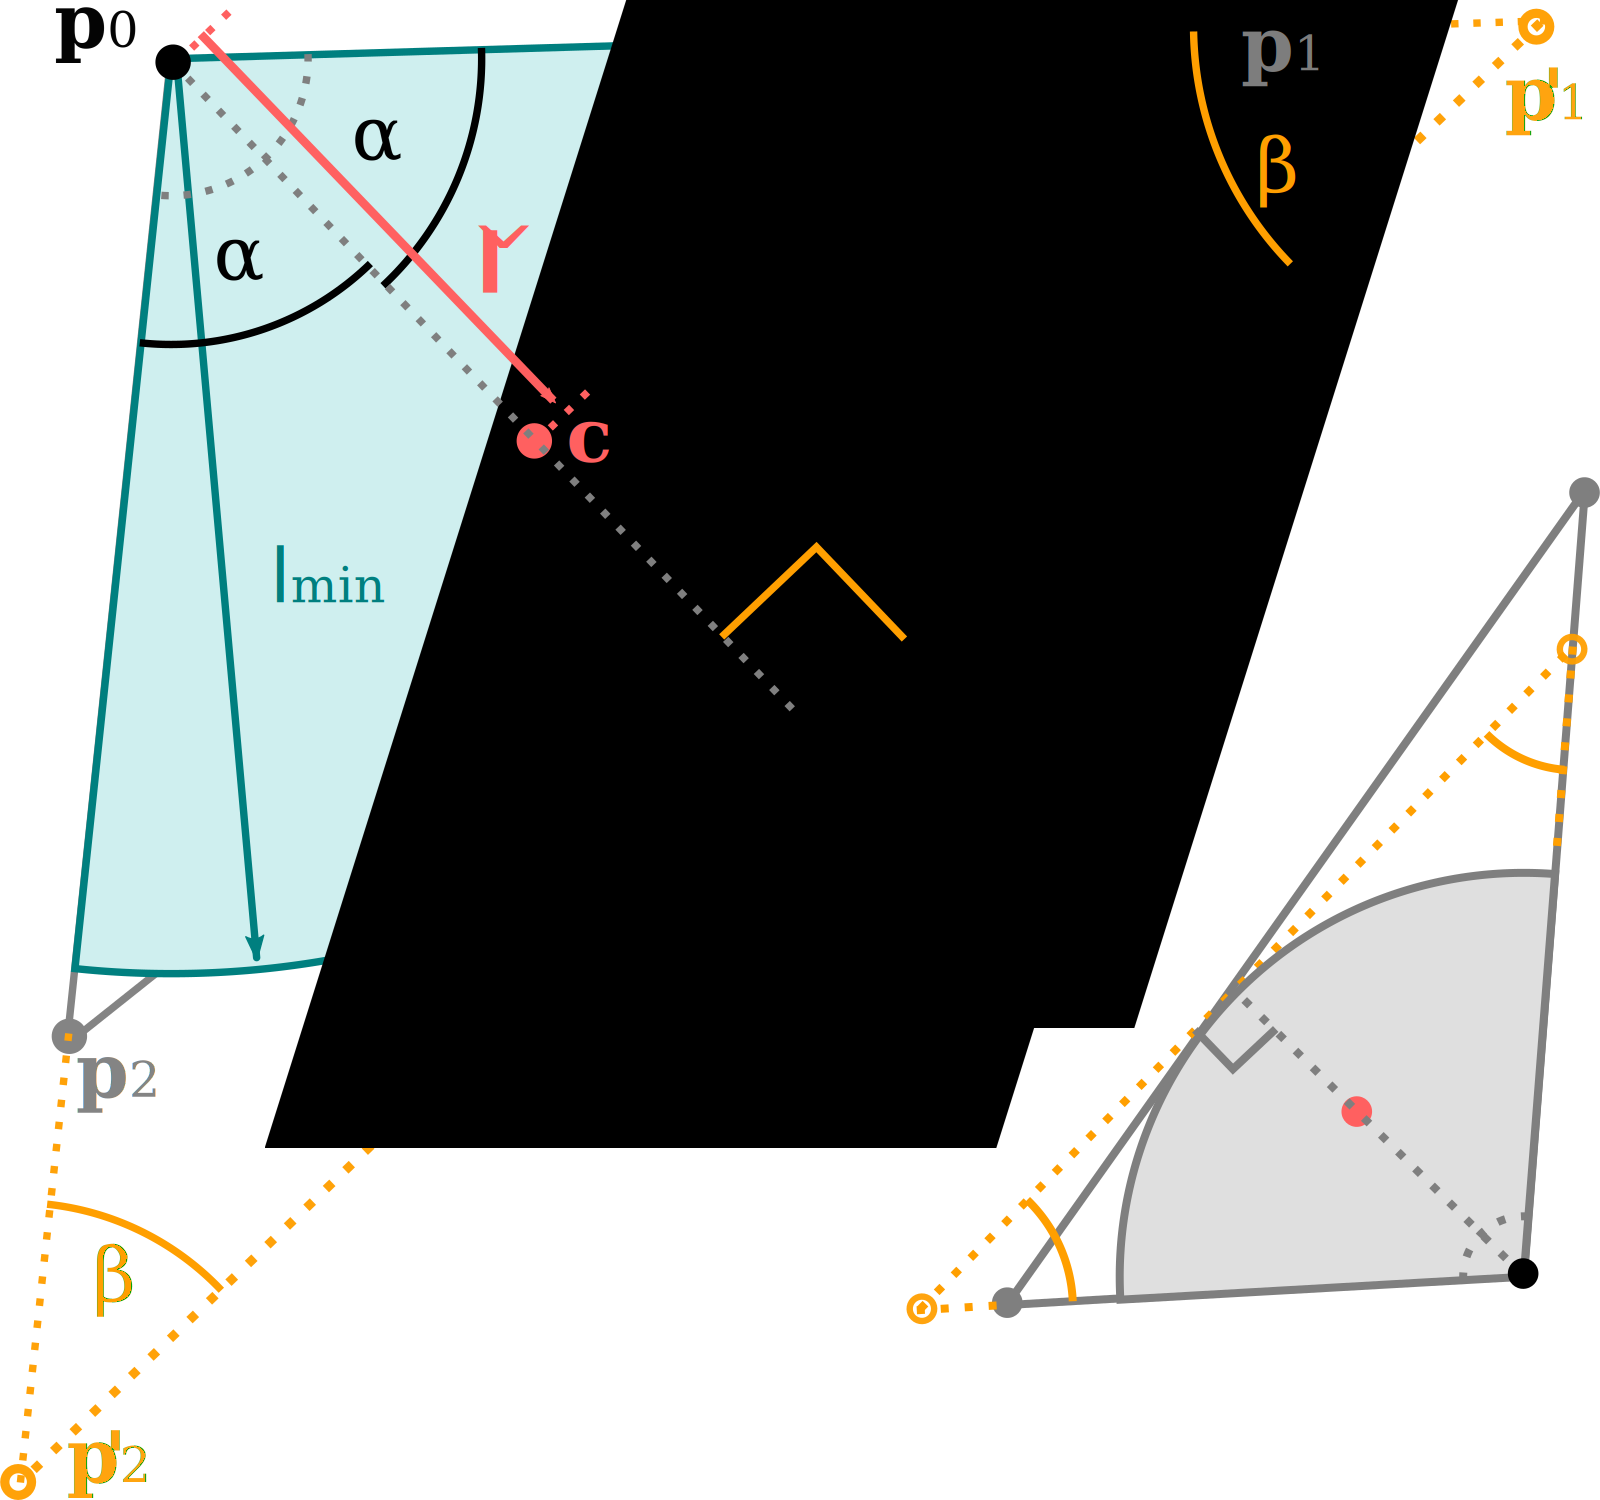
\includegraphics[width=0.5\linewidth]{../figures/anglesAndCenterOfGravity_presentation.png}
}

%------------------------------------------------
\frame{\frametitle{Interpolation of Function Values toward the Center of Gravity}
	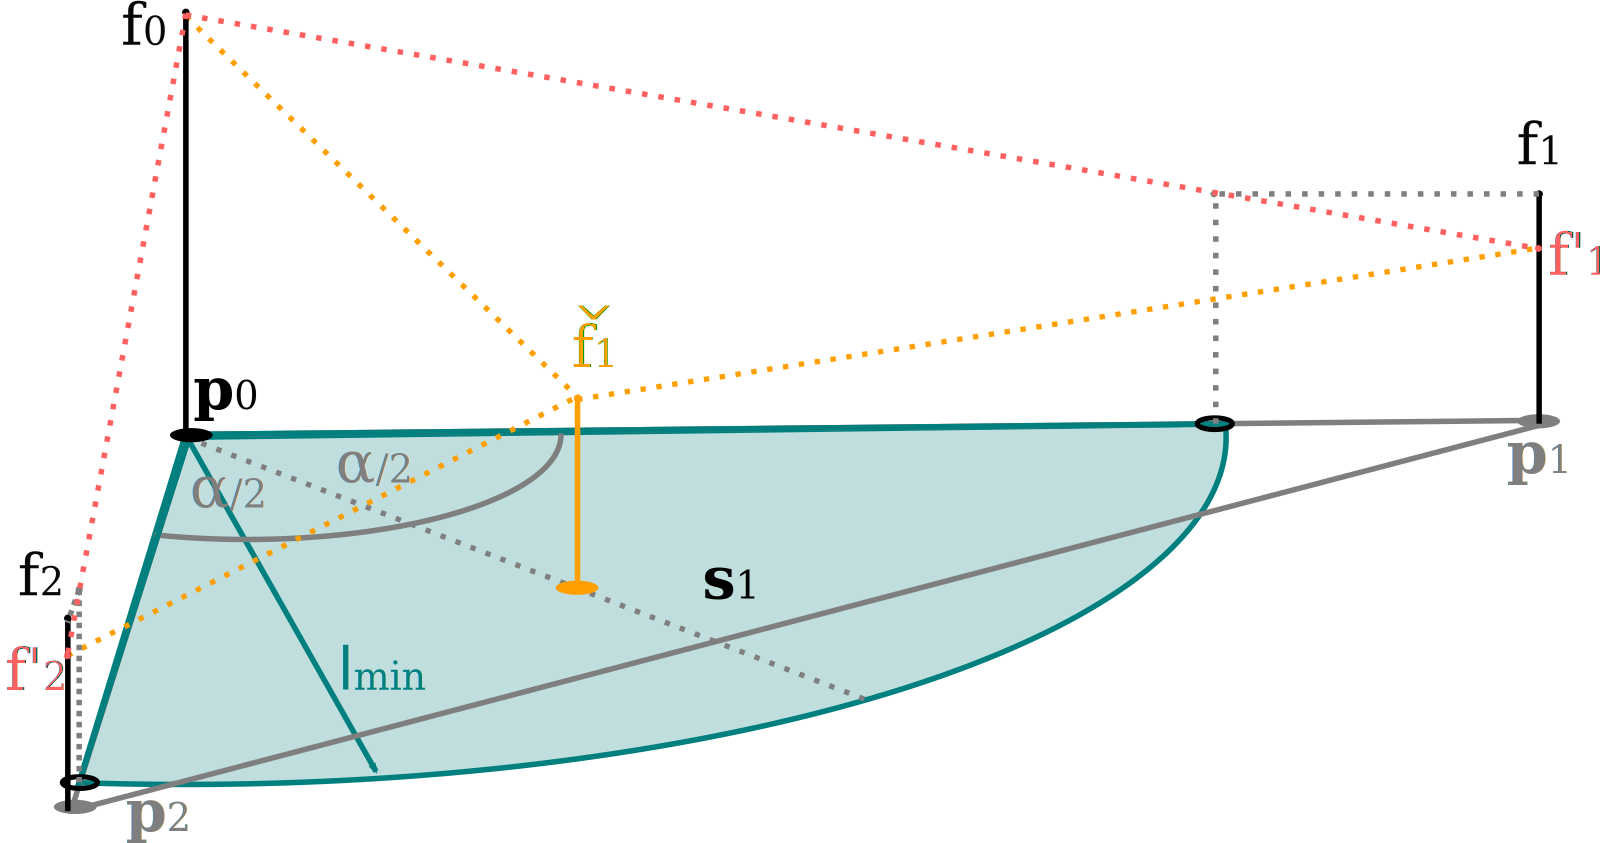
\includegraphics[width=1.0\linewidth]{../figures/interpolatedFunctionValues.png}
}

%------------------------------------------------
\frame{\frametitle{Weighted Mean Function Value $f'_v$at $\bp_v$}
	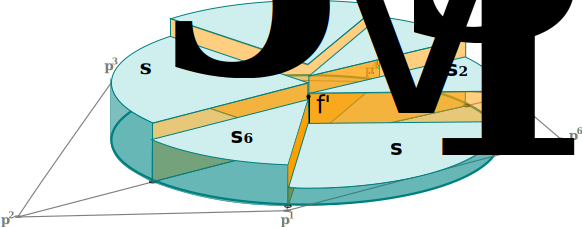
\includegraphics[width=1.0\linewidth]{../figures/funcValVolumes.png}
}


%================================================
\subsection[Serial]{Serial Algorithm}

%------------------------------------------------
\frame{\frametitle{Union Operations as Performed in Build Neighborhoods}
	\includestandalone[width=\textwidth]{../figures/tikz/unionsOfSimpleBuildNeighborhoods}
}

%------------------------------------------------
\frame{\frametitle{Serial Algorithm for Building Neighborhoods}
\begin{algorithm}[H]
	\SetAlgoSkip{}
	\DontPrintSemicolon
	\SetCommentSty{small}
	\SetKwFor{For}{for}{:}{}
	\SetKwProg{Func}{Function}{}{}
	\SetKwInOut{Input}{Input}\SetKwInOut{Output}{Output}

	\only<1>{
	\begin{block}{Part (1 of 2)}
		\Input{the set of all triangular faces $\bT$}
		\Output{the family of sets of discovered neighborhoods $\bN$}

		\bigskip
	\nl	\Func{serialBuildNeighborhoods($\bT$)}{\label{sbn1}
	\nl		\For(\tcc*[f]{$\bt = \left \{\bp_a, \bp_b, \bp_c\right \}$}){$\bt \in \bT$}{
	\nl			\ProgSty{union($\bN$, $\bp_a$, $\bp_b$, $\bp_c$)}\;
	\nl			\ProgSty{union($\bN$, $\bp_b$, $\bp_a$, $\bp_c$)}\;
	\nl			\ProgSty{union($\bN$, $\bp_c$, $\bp_a$, $\bp_b$)}\;
			}
		}
	\end{block}
	}

	\only<2>{
	\begin{block}{Part (2 of 2)}
	\nl	\Func{union($\bN$, $a$, $b$, $c$)}{
	\nl		$\bN_a \leftarrow \bN_a \cup \{b,\,c\}$\;
		}
	\end{block}
	}
\end{algorithm}
}

%------------------------------------------------
\frame{\frametitle{Serial Algorithm for Calculating Edge Lengths}
\begin{algorithm}[H]
	\SetAlgoSkip{}
	\DontPrintSemicolon
	\SetCommentSty{small}
	\SetKwFor{For}{for}{:}{}
	\SetKwProg{Func}{Function}{}{}
	\SetKwInOut{Input}{Input}\SetKwInOut{Output}{Output}

	\only<1>{
	\begin{block}{Part (1 of 1)}
		\Input{the set of all points $\bP$, \\
			the family of sets of discovered neighborhoods $\bN$}
		\Output{the set of pre-calculated edge lengths $\bE$, \\
			the global minimum edge length $\gelm$}

		\bigskip
	\nl	\Func{serialCalculateEdgeLengths($\bP$, $\bN$)}{
	\nl		\For{$\bp_v \in \bP$}{
	\nl			\For{$\bp_i \in \bN_v$}{
					\linespread{1.5}\selectfont
	\nl				$\bE_{\sv{i}} \leftarrow |\bp_i - \bp_v|$\tcc*[r]{This is $\ellstar$ as in Eq:~\ref{eq:localMinimumEdgeLength}}
	\nl				$\gelm \leftarrow \min\left \{\gelm,\,\bE_{\sv{i}}\right \}$\tcc*[r]{Eq:~\ref{eq:globalMinimumEdgeLength}}
				}
			}
		}
	\end{block}
	}
\end{algorithm}
}

%------------------------------------------------
\frame{\frametitle{Serial Algorithm for Convolving the Filter}
\begin{algorithm}[H]
	\SetAlgoSkip{}
	\DontPrintSemicolon
	\SetCommentSty{small}
	\SetKwFor{For}{for}{:}{}
	\SetKwProg{Func}{Function}{}{}
	\SetKwProg{Cont}{}{}{}
	\SetKwInOut{Input}{Input}\SetKwInOut{Output}{Output}

	\only<1>{
	\begin{block}{Part (1 of 4)}
		\Input{the set of all points $\bP$, \\
			the family of sets of discovered neighborhoods $\bN$, \\
			the set of pre-calculated edge lengths $\bE$, \\
			the global minimum edge length $\gelm$, \\
			the set of function values $\bF$, \\
			the user-defined number of convolutions $\tau$}
		\Output{the set of one-ring \wmfv{s} $\bF'$}

		\bigskip
		\linespread{1}\selectfont
	\nl	\Func{serialConvolveFilter($\bP$, $\bN$, $\bE$, $\gelm$, $\bF$, $\tau$)}{
			\emph{(Continued\ldots)}
		}
	\end{block}
	}

	\only<2>{
	\setcounter{AlgoLine}{0}
	\begin{block}{Part (2 of 4)}
	\nl	\Func{serialConvolveFilter($\bP$, $\bN$, $\bE$, $\gelm$, $\bF$, $\tau$)}{
	\nl		\For{$t\leftarrow 1\;\KwTo\;\tau$}{
	\nl			\For{$\bp_v \in \bP$}{
	\nl				\For{$\bp_i \in \bN_v$}{
						\linespread{1.5}\selectfont
	\nl					$\kern-0.5pt\alpha \leftarrow cos^{-1}$
						\begin{Large}
							$\kern-6pt\left (\frac{\bE_c^2\,+\,\bE_b^2\,-\,\bE_a^2}{2\,\cdot\,\bE_c\,\cdot\,\bE_b}\right )$\tcc*[r]{Eq:~\ref{eq:alphaFromEdgeLengths}}
						\end{Large}\label{algSCFalpha}
						\linespread{1.2}\selectfont
	\nl					$\kern0.00pt\beta \leftarrow (\pi - \alpha)\mathbin{/}2$\tcc*[r]{Eq:~\ref{eq:betaFromHalfAlpha}}\label{algSCFbeta}
	\nl					$\kern-1.5ptA \leftarrow \Big(\gelm\,\Big)^2\kern-4pt\cdot\alpha\mathbin{/}2$\tcc*[r]{Eq:~\ref{eq:circularSectorArea}}\label{algSCFarea}
					}
				}
			}
		}
	\end{block}
	}
	\only<3>{
	\setcounter{AlgoLine}{0}
	\begin{block}{Part (3 of 4)}
		\Cont{}{
			\vspace*{-1\baselineskip}
			\Cont{}{
				\vspace*{-1\baselineskip}
				\Cont{}{
					\vspace*{-1\baselineskip}
					\Cont{}{
	\nl					$\kern1.00pt\check{\ell} \leftarrow \big(4\cdot\gelm\cdot\sin(\alpha\mathbin{/}2)\big)\mathbin{/}3\,\alpha$\tcc*[r]{Eq:~\ref{eq:distToCoG}\enspace\footnotemark{}}\label{algSCFcog}
	\nl					$\kern1.00pt\zeta \leftarrow \gelm\mathbin{/}\sin(\beta)$\tcc*[r]{Eq:~\ref{eq:zeta}}\label{algSCFzeta}
	\nl					\For{$j \in {1,2}$}{\label{algSCFjloop}
	\nl						$\tilde{\ell}_j \leftarrow \zeta\mathbin{/}\bE_j$\tcc*[r]{Eq:~\ref{eq:distanceIForInterpolation},~\ref{eq:distanceIp1ForInterpolation}}
	\nl						$f'_j \leftarrow f_0\cdot(1 - \tilde{\ell}_j) + f_j\cdot\tilde{\ell}_j$\tcc*[r]{Eq:~\ref{eq:interpolatedFi},~\ref{eq:interpolatedFip1}}
						}
	\nl					$\check{f} \leftarrow f_0\cdot(1 - \check{\ell}) + \big((f'_1 + f'_2)\cdot\check{\ell}\big)\mathbin{/}2$\tcc*[r]{Eq:~\ref{eq:weightedMeanAtCoGatSector}}\label{algSCFcheckf}
					}
				}
			}
		}
	\end{block}
	}
	\only<4>{
	\setcounter{AlgoLine}{0}
	\begin{block}{Part (4 of 4)}
		\Cont{}{
			\vspace*{-1\baselineskip}
			\Cont{}{
				\vspace*{-1\baselineskip}
				\Cont{}{
					\vspace*{-1\baselineskip}
					\Cont{}{
	\nl					$\kern-2.0pt\tilde{f}_v \leftarrow \tilde{f}_v + A\cdot\check{f}$\tcc*[r]{Eq:~\ref{eq:meanFuncValAtPv}}\label{algSCFtildef}
	\nl					$\kern-4.0pt\tilde{A}_v \leftarrow \tilde{A}_v + A$\tcc*[r]{Eq:~\ref{eq:meanFuncValAtPv}}\label{algSCFtildeA}
					}
	\nl				$f'_v \leftarrow \tilde{f}_v\mathbin{/}\tilde{A}_v$\tcc*[r]{Eq:~\ref{eq:meanFuncValAtPv}}\label{algSCFfprimev}
				}
	\nl		$\bF' \leftarrow \left \{f'_1,\ldots,\,f'_{|\bP|}\right \}$\;\label{algSCF2ndlastLine}
	\nl 	$\bF \leftarrow \bF'$\tcc*{smooth newest values every convolution}\label{algSCFlastLine}
			}
		}
	\end{block}
	}
\end{algorithm}
}


%================================================
\subsection[Parallel]{Parallel Algorithm}

%------------------------------------------------
\frame{\frametitle{Parallel Algorithm}
}




%================================================
%================================================
\section{Experiments \& Evaluation}


%================================================
\subsection{Filter Response}

%------------------------------------------------
\frame{
\frametitle{Experiment 1}

}


%================================================
\subsection{Parallel Algorithm}

%------------------------------------------------
\frame{\frametitle{Evaluation and Analysis of Parallel Algorithms}

\begin{align}
	\mathit{T_s}(\hat{n}) &= \text{The optimal sequential execution time} \\
	\mathit{T_{\rho}}(\hat{n},\,\rho) &= \text{Parallel runtime}
	\label{eq:timings}
\end{align}

which can then be used to define the three essential metrics:

\begin{align}
	\text{Speedup:}\quad&\mathit{S}(\hat{n},\,\rho) = \frac{\mathit{T_s}(\hat{n})}{\mathit{T_{\rho}}(\hat{n},\,\rho)} \\
	\text{Costs}:\quad&\mathit{C}(\hat{n},\,\rho) =\rho\cdot\mathit{T_{\rho}}(\hat{n},\,\rho) \\
	\text{Efficiency}:\quad&\mathit{E}(\hat{n},\,\rho) = \frac{\mathit{T_s}(\hat{n})}{\mathit{C}(\hat{n},\,\rho)} = \frac{\mathit{S}(\hat{n},\,\rho)}{\rho}
	\label{eq:essentialMetrics}
\end{align}
}

%------------------------------------------------
\frame{\frametitle{Amdahl's law and the Degree of Parallelism}
Also important is the notion of an algorithm's ``degree of parallelism'', which is the maximum number of operations that can be executed in parallel, a principle central to Amdahl's law~\cite{Amdahl67} which is defined as, when given a constant problem size $\hat{n}_{fixed}$, and an algorithm's degree of parallelism $q$,

\begin{equation}
	\lim_{\rho \to \infty} \mathit{S}(\hat{n}_{fixed},\,\rho) = 1 / q
\end{equation}

This leads to the conclusion that one can not simply add more processors in order to gain appreciable speedup, but instead that relies heavily on processor counts which grow in relation to problem sizes, and the degree of parallelism, which itself relies on the underlying nature of the serial algorithm and the artful design of the parallel algorithm.
}



%================================================
%================================================
\section[Conclusion]{Conclusion \& Outlook}

%------------------------------------------------
\frame{
\frametitle{Conclusion}

}

%------------------------------------------------
\frame{
\frametitle{Outlook}

}

%------------------------------------------------
\frame{\frametitle{Questions}
	
\includegraphics[width=.8\textwidth]{questions}
	\vspace*{-3.3cm}
	\begin{center}
		\begin{LARGE}
			\textbf{Questions}
		\end{LARGE}
	\end{center}
	\vspace*{2cm}
}

\end{document}
